%% MODELO DE LATEX PARA TRABALHOS ACADÊMICOS
%% INSTRUÇÕES GERAIS:
%%    1. TODO O TEXTO NA FRENTE DO SIMBOLO '%' É COMENTÁRIO, ISTO É, ELE NÃO FAZ DIFERENÇA NO RESULTADO FINAL 
%%    2. NESTE MODELO, VOCÊS SÓ PRECISAM EDITAR DAS LINHAS 114 A 132 (INFORMAÇÕES DE CAPA) E DAS LINHAS 188 EM DIANTE (CORPO DO TRABALHO). O RESTO SÃO CONFIGURAÇÕES DE FORMATAÇÃO QUE PROVAVELMENTE NÃO SERÁ PRECISO MODIFICAR.
%%    3. MAIS INSTRUÇÕES DETALHADAS PODERÃO SER ENCONTRADAS NA PÁGINA profhelioh.wordpress.com. DÚVIDAS: heliohenrique@ufpr.br OU heliohenrique3@gmail.com

% INFORMAÇÕES DA FONTE:
%% abtex2-modelo-relatorio-tecnico.tex, v-1.7.1 laurocesar
%% Copyright 2012-2013 by abnTeX2 group at http://abntex2.googlecode.com/ 
%%
%% This work may be distributed and/or modified under the
%% conditions of the LaTeX Project Public License, either version 1.3
%% of this license or (at your option) any later version.
%% The latest version of this license is in
%%   http://www.latex-project.org/lppl.txt
%% and version 1.3 or later is part of all distributions of LaTeX
%% version 2005/12/01 or later.
%%
%% This work has the LPPL maintenance status `maintained'.
%% 
%% The Current Maintainer of this work is the abnTeX2 team, led
%% by Lauro César Araujo. Further information are available on 
%% http://abntex2.googlecode.com/
%%
%% This work consists of the files abntex2-modelo-relatorio-tecnico.tex,
%% abntex2-modelo-include-comandos and abntex2-modelo-references.bib
%%
% ------------------------------------------------------------------------
% ------------------------------------------------------------------------
% abnTeX2: Modelo de Relatório Técnico/Acadêmico em conformidade com 
% ABNT NBR 10719:2011 Informação e documentação - Relatório técnico e/ou
% científico - Apresentação
% ------------------------------------------------------------------------ 
% ------------------------------------------------------------------------

\documentclass[
	% -- opções da classe memoir --
	12pt,				% tamanho da fonte
	% openright,			% capítulos começam em pág ímpar (insere página vazia caso preciso)
    oneside,			% para impressão somente frente. Oposto a twoside (frente e verso)
	a4paper,			% tamanho do papel. 
	% -- opções da classe abntex2 --
	%chapter=TITLE,		% títulos de capítulos convertidos em letras maiúsculas
	%section=TITLE,		% títulos de seções convertidos em letras maiúsculas
	%subsection=TITLE,	% títulos de subseções convertidos em letras maiúsculas
	%subsubsection=TITLE,% títulos de subsubseções convertidos em letras maiúsculas
	% -- opções do pacote babel --
	english,			% idioma adicional para hifenização
	french,				% idioma adicional para hifenização
	spanish,			% idioma adicional para hifenização
	brazil,				% o último idioma é o principal do documento
	]{abntex2}


% ---
% PACOTES
% ---

% ---
% Pacotes fundamentais 
% ---

\usepackage{cmap}				% Mapear caracteres especiais no PDF
\usepackage{lmodern}			% Usa a fonte Latin Modern
\usepackage[T1]{fontenc}		% Selecao de codigos de fonte.
\usepackage[utf8]{inputenc}		% Codificacao do documento (conversão automática dos acentos)
\usepackage{indentfirst}		% Indenta o primeiro parágrafo de cada seção.
\usepackage{color}				% Controle das cores
\usepackage{graphicx}			% Inclusão de gráficos
\usepackage{url}

% ---
\expandafter\def\expandafter\UrlBreaks\expandafter{\UrlBreaks%  save the current one
  \do\a\do\b\do\c\do\d\do\e\do\f\do\g\do\h\do\i\do\j%
  \do\k\do\l\do\m\do\n\do\o\do\p\do\q\do\r\do\s\do\t%
  \do\u\do\v\do\w\do\x\do\y\do\z\do\A\do\B\do\C\do\D%
  \do\E\do\F\do\G\do\H\do\I\do\J\do\K\do\L\do\M\do\N%
  \do\O\do\P\do\Q\do\R\do\S\do\T\do\U\do\V\do\W\do\X%
  \do\Y\do\Z}



%%%
\usepackage{float}

%Incluir Fonte a figuras e tabelas.
\newcommand{\source}[1]{\caption*{Fonte: {#1}} }

%% Gerenciamento do numeração de equações
\usepackage{amsmath}

%%%
% ---
% Pacotes adicionais, usados no anexo do modelo de folha de identificação
% ---
\usepackage{multicol}
\usepackage{multirow}
% ---
	
% ---
% Pacotes adicionais, usados apenas no âmbito do Modelo Canônico do abnteX2
% ---
\usepackage{lipsum}				% para geração de dummy text
% ---

% ---
% Pacotes de citações
% ---
\usepackage[brazilian,hyperpageref]{backref}	 % Paginas com as citações na bibl
\usepackage[alf]{abntex2cite}	% Citações padrão ABNT
\hiddenbibitem
% --- 
% CONFIGURAÇÕES DE PACOTES
% --- 

% ---
% Configurações do pacote backref
% Usado sem a opção hyperpageref de backref
\renewcommand{\backrefpagesname}{Citado na(s) página(s):~}
% Texto padrão antes do número das páginas
\renewcommand{\backref}{}
% Define os textos da citação
\renewcommand*{\backrefalt}[4]{
	\ifcase #1 %
		Nenhuma citação no texto.%
	\or
		Citado na página #2.%
	\else
		Citado #1 vezes nas páginas #2.%
	\fi}%
% ---
%Local das imagens
\graphicspath{ {Figuras/} }
% ---
% Informações de dados para CAPA e FOLHA DE ROSTO
% ---
\titulo{Classificação automática de situações em tráfego de veículos}
\autor{ARTHUR AMARAL DE OLIVEIRA}
\local{São Bernardo do Campo}
\data{10 de Setembro, 2018}
\instituicao{%
  CENTRO UNIVERSITÁRIO FEI}
\tipotrabalho{Relatório técnico}
% O preambulo deve conter o tipo do trabalho, o objetivo, 
% o nome da instituição e a área de concentração 
\preambulo{Qualificação de Mestrado apresentada ao Centro Universitário da FEI, como parte dos requisitos necessários para obtenção do título de Mestre em Engenharia Elétrica, orientado pelo Prof. Dr. Paulo Eduardo Santos.}
% ---

% ---
% Configurações de aparência do PDF final

% alterando o aspecto da cor azul
\definecolor{blue}{RGB}{41,5,195}

% informações do PDF
\makeatletter
\hypersetup{
     	%pagebackref=true,
		pdftitle={\@title}, 
		pdfauthor={\@author},
    	pdfsubject={\imprimirpreambulo},
	    pdfcreator={LaTeX with abnTeX2},
		pdfkeywords={abnt}{latex}{abntex}{abntex2}{relatório técnico}, 
		colorlinks=true,       		% false: boxed links; true: colored links
    	linkcolor=blue,          	% color of internal links
    	citecolor=blue,        		% color of links to bibliography
    	filecolor=magenta,      		% color of file links
		urlcolor=blue,
		bookmarksdepth=4
}
\makeatother
% --- 

% --- 
% Espaçamentos entre linhas e parágrafos 
% --- 

% O tamanho do parágrafo é dado por:
\setlength{\parindent}{1.3cm}

% Controle do espaçamento entre um parágrafo e outro:
\setlength{\parskip}{0.2cm}  % tente também \onelineskip

% ---
% compila o indice
% ---
\makeindex
% ---

% ----
% Início do documento
% ----
\begin{document}

% Retira espaço extra obsoleto entre as frases.
\frenchspacing 

% ----------------------------------------------------------
% ELEMENTOS PRÉ-TEXTUAIS
% ----------------------------------------------------------
% \pretextual

% ---
% Capa
% ---
\imprimircapa
% ---

% ---
% Folha de rosto
% (o * indica que haverá a ficha bibliográfica)
% ---
\imprimirfolhaderosto*
% ---


% ---
% Agradecimentos
% ---
%\begin{agradecimentos}
%O agradecimento principal é direcionado a Youssef Cherem, autor do
%\nameref{formulado-identificacao} (\autopageref{formulado-identificacao}).

%Os agradecimentos especiais são direcionados ao Centro de Pesquisa em
%Arquitetura da Informação\footnote{\url{http://www.cpai.unb.br/}} da Universidade de
%Brasília (CPAI), ao grupo de usuários
%\emph{latex-br}\footnote{\url{http://groups.google.com/group/latex-br}} e aos
%novos voluntários do grupo
%\emph{\abnTeX}\footnote{\url{http://groups.google.com/group/abntex2} e
%\url{http://abntex2.googlecode.com/}}~que contribuíram e que ainda
%contribuirão para a evolução do abn\TeX.

%\end{agradecimentos}
% ---

% ---
% RESUMO
% ---

% resumo na língua vernácula (obrigatório)
\begin{resumo} %% AQUI COMEÇA A PÁGINA DE RESUMO
O raciocínio probabilístico utilizando-se da teoria das probabilidades nos oferece recursos para codificar as incertezas de um contexto quantitativamente. Este trabalho apresentará um sistema de assistência ao motorista que utilizará evidências obtidas a partir da classificação de uma série de quadros de um contexto de tráfego de veículos por uma rede neural convolucional, e em conjunto com uma base de conhecimento que conterá regras do Código Brasileiro de Trânsito, calculará a probabilidade de colisão de veículos.


 \vspace{\onelineskip}
    
 \noindent
 \textbf{Palavras-chaves}: raciocínio probabilístico, redes neurais convolucionais.
\end{resumo} %AQUI TERMINA A PÁGINA DE RESUMO
% ---

% ---
% inserir lista de ilustrações
% ---

%  \listoffigures* %% o * indica que não será incluso no sumário
%  \cleardoublepage %% Pula página
% ---

% ---
% inserir lista de tabelas
% ---

%  \listoftables*
%  \cleardoublepage
% ---

% ---
% inserir lista de abreviaturas e siglas
% ---
%\begin{siglas}
%  \item[Fig.] Area of the $i^{th}$ component
%  \item[456] Isto é um número
%  \item[123] Isto é outro número
%  \item[lauro cesar] este é o meu nome
%\end{siglas}
% ---

% ---
% inserir lista de símbolos
% ---
%\begin{simbolos}
%  \item[$ \Gamma $] Letra grega Gama
%  \item[$ \Lambda $] Lambda
%  \item[$ \zeta $] Letra grega minúscula zeta
%  \item[$ \in $] Pertence
%\end{simbolos}
% ---

% ---
% inserir o sumario
% ---

\tableofcontents*

% ---

% ----------------------------------------------------------
% ELEMENTOS TEXTUAIS  (necessário para incluir número nas páginas)
% ----------------------------------------------------------
\textual


% ----------------------------------------------------------
% Introdução
% ----------------------------------------------------------
\chapter{Introdução} %% NOVO CAPÍTULO (REPARE QUE ELE AUTOMATICAMENTE JÁ COLOCA O NÚMERO DO CAPÍTULO E JÁ ADICIONA NO SUMÁRIO)

De acordo com o programa Europeu de avaliação carros novos, cuja sigla Euro NCAP vem do inglês "European New Car Assessment Programme", em seu estudo \citeonline{EURONCAP2025}, cita que 90\% dos acidentes são causados por erros de humanos. Em geral são dois problemas que  contribuem para que os erros aconteçam. O primeiro está ligado às violações das regras de trânsito, como velocidade acima do permitido, direção sobre influência de drogas ou álcool; o segundo está relacionado à falta de atenção ao trânsito, fatiga, distração e a inexperiência do motorista. 

Como resposta ao segundo problema, a indústria automotiva tem desenvolvido diversos sistemas de auxilio a direção, em Inglês "Advanced Driver Assistance Systems" (ADAS) para dar suporte ao motorista para que previnam e mitiguem os erros causados por humanos na condução de seus veículos. Os principais sistemas hoje são o sistemas de aviso de troca de faixa, assistência para se manter dentro da faixa, sistemas autônomos de emergência de mudança de direção, piloto automático adaptativo, sistemas de assistência de velocidade, entre outros. 

Segundos estudo da Organização Mundial de Saúde, conforme mostrado em \citeonline{8429957}, 1,25 milhões de mortes ocorre todo ano com acidentes relacionados ao trafego de veículos, e monetariamente isso significa um gasto anual de  US\$ 518 bilhões. Este dados além da crescente demanda por segurança dos motorista, fizeram que os fabricantes de automóveis desenvolver sistemas avançados de auxílio a direção de veículos. 

Para poder representar o contexto de tráfego de veículos as técnicas de Aprendizado de Máquina, mais precisamente as Redes Neurais Artificias (RNA) e em especial Redes Neurais Convolucionais (RNC), tem nos últimos anos obtidos grandes resultados no campo da visão computacional em detectar, classificar e segmentar objetos. Ano após ano os resultados obtidos no desafio de detecção e classificação de objetos proposto pela \textit{ImageNet}, base de dados mais de 14 milhões de imagens \citeonline{Deng09imagenet}, mostram os avanços conseguidos pelas RNC's.

Apesar do grande crescimento dos sistemas de Aprendizado de Máquina, as Redes Neurais não conseguem interpretar o contexto como um todo, mas sim mostrar todos os objetos que compõem aquele contexto. A interpretação do contexto e suas incertezas necessitam que existam  regras e relações espaço-temporais. O Raciocínio Probabilístico, utilizando-se regras de Lógica escritas Lógica Probabilística é uma técnica apropriada para modelar este contexto. De acordo com \citeonline{phdthesis_problog}, aplicações que necessitam de um maior formalismo devido ao raciocínio sobre incertezas precisam mais do que apenas lógica, por essa razão uma vasta quantidade de desenvolvimentos foram feitos na área de Programação em Lógica Probabilística. $ProbLog$ é uma ferramenta de Programação de Lógica Probabilística que é uma extensão do $Prolog$, que além de Lógica Booleana pode receber também sentenças em Lógica de Primeira Ordem.

Este trabalho propõe um sistema ADAS que utilizará Redes Neurais Convolucionais, utilizando uma sequência de quadros de uma cena de tráfego de veículos como entrada, e obter na sua saída uma lista classificada com as probabilidade dos objetos detectados estarem na cena. Esta lista será utilizada como evidências para um sistema de raciocínio probabilístico, que será escrito em $ProbLog$ que é uma ferramenta de programação em lógica probabilística. Este programa conterá regras de ultrapassagens descritas no Código Brasileiro de Trânsito que também serão codificadas em $ProbLog$, utilizando-se tanto as regras de trânsito quanto as evidências providas pela RNC será possível inferir se uma cena apresenta possíveis situações de colisão entre veículos.

%

% ---
% Capitulo de revisão de literatura
% ---
\chapter{Revisão Bibliográfica}

Nas áreas de Raciocínio Lógico e Aprendizado de Máquina, existem diversos trabalhos que mostram técnicas utilizadas para inferência, localização, classificação e reconhecimento de padrões em imagens e vídeos.

\section {Redes Neurais Artificiais}

\citeonline{NIPS2012_4824} propuseram uma RNC que consiste em 5 camadas convolucionais, entre elas existem algumas camadas de agrupamento máximo e três camadas totalmente conectadas. O uso da RNC foi escolhido ao invés de  Redes Neurais de alimentação avante ou alimentação direta com camadas de tamanhos similares, porque as RNC's podem utilizar muito menos conexões e parâmetros, além de serem mais facilmente treinadas e com apenas uma pequena perda de performance. Esta proposta contribuiu com um maneira eficiente e altamente otimizada de realizar a convolução das imagens em 2D utilizando-se de duas unidades de processamento gráfico (UPG), além disso a comunicação entre as UPG não é realizada em todas as camadas. Outra contribuição foi a não utilização da forma tradicional de modelagem das saídas dos neurônios (saturação não-linear), foram utilizadas as funções retificadas lineares (FRL), que tem a  importante propriedade de não necessitar de normalização para prevenir que o processo de aprendizado continue, quando um exemplo já gerou uma entrada positiva. Alternativas aos modelos tradicionais também foram mencionadas em Jarret et. al (2009). 

No trabalho proposto por \citeonline{DBLP:journals/corr/SzegedyLJSRAEVR14} para participar do "ImageNet Large-Scale Visual Recognition Challenge" (ILSVRC) de 2014, uma RNC chamada de \textit{Inception} foi melhorada sem que houvesse acréscimo computacional. Para manter a computação inalterada, foram introduzidas camadas esparsas ao invés de camadas totalmente conectadas, inclusive dentro das camadas de convolução, ainda que o estado da arte atual na visão computacional esteja usando camadas totalmente conectadas. O ganho introduzido pelas camadas esparsas acontece se a distribuição de probabilidades do conjunto de dados for representada por rede neural esparsa. Dessa maneira uma topologia de rede ótima pode ser construída, camada a camada. Analisando-se  as correlações estatísticas das ativações dos neurônios em camadas anteriores, e agregando-se os neurônios  com alta correlação na saída,  segundo \citeonline{DBLP:journals/corr/SzegedyLJSRAEVR14} esta afirmação se aproxima do Princípio de Hebbian, “Neurônios que disparam juntos permanecem conectados”. 

No trabalho apresentado por \citeonline{DBLP:journals/corr/SimonyanZ14a} para a competição de ILSVRC de 2015 foi proposta uma RNC com 19 camadas, que segue o mesmo princípio de aumentar a profundidade da RNC assim como em Szegedy et. al (2015), entretanto o resultado foi melhor em termos de localização de objetos. Diferentemente de \citeonline{DBLP:journals/corr/SzegedyLJSRAEVR14}, \citeonline{DBLP:journals/corr/SimonyanZ14a} usaram uma estrutura de rede mai simples.

O gargalo computacional atual da detecção de objetos através de RNC, segundo \citeonline{DBLP:journals/corr/RenHG015} é o região, dentro da imagem, onde a RNC irá analisar a detecção de objetos, por esta razão, \citeonline{DBLP:journals/corr/RenHG015} propuseram uma RNC chamada de "Faster R-CNN". Para a geração de regiões, uma RNC’s totalmente conectada é treinada para detectar os limites dos objetos e uma pontuação do objeto para cada posição. A saída da camada convolucional, gera um mapa de características que são usadas tanto para gerar as regiões propostas de localização dos objetos, quanto como entrada para uma outra RNC para a atividade de detecção. Por esta razão as propostas de regiões tem custo computacional quase zero. Este custo baixo de computação é obtido pelo treinamento das redes, primeiro é treinada a RNC com a ImageNet para a tarefa de gerar as propostas de regiões, e depois é treinada utilizando-se a as proposta geradas pela RNC. Depois dessa etapa, as camadas de convolução ainda não estão conectadas, o último passo é fazer a conexão entre as redes. Esta proposta de detecção de objetos consegue ser eficiente com uma taxa de 5-17 quadros por segundo.

\citeonline{taylor-eccv-10} desenvolveram um método capaz de aprender representações de uma sequência de pares de sucessivas imagens usando fluxo ótico como entrada para a RNC, e foi possível extrair características de movimento, segmentação e detecção de bordas. Uma diferença entre outros método propostos durante seu estudo foi a introdução de probabilidades na camada que realiza o agrupamento pelo valor máximo. 

Combinando RNC com o algoritmo de análise independente do subespaço (ISA) \citeonline{Le:2011:LHI:2191740.2192108} mostram que é possível identificar variações temporais em vídeos. Nas primeiras camadas da RNC, o modelo aprende características que detectam movimentos de borda. Através da variação da velocidade dos objetos na imagem com a aplicação do ISA, obtêm-se neurônios altamente sensíveis a variação da velocidade. Esta propriedade faz com que essa abordagem seja capaz de reconhecer movimentos.

A classificação de imagens por RNC apresentou grandes resultados como descrito anteriormente, essa razão motivou  \citeonline{KarpathyCVPR14} em avaliar a utilização de RNC’s para classificação de vídeos e compará-la com as melhores práticas de classificação de algoritmos baseados em características locais, seus resultados mostram que a performance do uso de RNC tem melhores resultados. \citeonline{KarpathyCVPR14} apresentaram também um método que utiliza uma arquitetura com duas RNC’s que processa separadamente a entrada em duas diferentes resoluções espaciais, que são fundidas na primeira camada totalmente conectada. Para agregar a informação de tempo, são agregadas informações de 10 quadros e então são submetidos a todos os níveis convolucionais. Os quadros da entrada são reduzidos pela metade em sua resolução espacial. Para a primeira RNC esta é a imagem de entrada, já para a segunda, valendo-se da premissa que a o objeto de interesse ocupa a região central da imagem, a segunda RNC somente recebe a porção central do objeto. Essa redução de resolução não prejudicou o resultado final do experimento e ainda houve redução de 50\% no tempo de treinamento. 

\citeonline{NIPS2014_5353} propõem um novo método para reconhecimento de ações em vídeos, que consistem em analisar separadamente a parte espacial e a temporal de uma sequência de quadros. A parte espacial, traz informações sobre a cena e seus objetos a cada quadro, a sequência de quadros traz informações sobre o movimento da cena, da câmera e ainda movimento dos objetos presentes na cena. A análise espacial e a temporal são implementadas separadamente usando RNC’s e classificação normalizada entre 0 e 1. O processo da análise da parte espacial não contempla nenhuma novidade, entretanto na análise temporal, a entrada para a RNC é a variação do fluxo ótico ou variação de trajetória, em uma sequência consecutiva de quadros. Dessa maneira os dados de entrada já representam um movimento, não sendo necessário que a RNC avaliem se existe ou não movimento. Para agregar os resultados das duas RNC’s foram utilizados dois métodos, a média e máquina de vetores de suporte (SVM) sobre o resultado normalizado da segunda camada de classificação.

Além das RNC’s serem usadas em uma ampla lista de tarefas utilizando-se imagens como entrada, em  \citeonline{DBLP:journals/corr/RavanbakhshMRMD15} são utilizados vídeos ao invés de apenas imagens com o objetivo de reconhecimento de ações. Utilizando-se a última camada de RNC antes da camada de classificação, \citeonline{DBLP:journals/corr/RavanbakhshMRMD15} introduziu uma estrutura hierárquica capaz de capturar a variação temporal em vídeos, este modelo foi capaz de capturar pequenas ações dentro de ações complexas, essas pequenas ações representam um grau diferente de granularidade dentro da ação completa. A estrutura foi proposta capturando-se as características espaciais usando a arquitetura AlexNet \citeonline{NIPS2012_4824}, sendo treinadas com a base de dados ImageNet. As características temporais, diferentemente dos trabalhos anteriores que propunham fluxo óptico, foram adquiridas utilizando-se pequenos intervalos do vídeo. N nesse intervalo, são computadas informações grosseiras das características dos quadros iniciais e finais, então o intervalo é dividido recursivamente, e são computadas novamente as características até que não seja mais possível dividir o intervalo do vídeo. Essas informações formam uma estrutura de árvore binária onde os níveis mais perto da raiz representam as informações mais grosseiras ao mesmo tempo que mais perto das folhas tem-se as características mais finas do movimento. Para a análise da estrutura de árvore binária foi utilizada a abordagens clássicas da visão computacional . O método de classificação proposto foi SVM não linear.

Em \citeonline{DBLP:journals/corr/abs-1708-02349}, foi apresentada uma nova abordagem para o reconhecimento de ações em vídeos, é explicado que ações são definidas por atividade de curto espaço de tempo, enquanto uma atividade é um conjunto de ações, e este conjunto de ações é o foco do seu estudo. Para uma precisa localização de atividades humanas foi proposta uma Rede de Contexto Temporal (TCN). Esta rede é similar a uma rede do tipo Rede Neural Convolucional baseada em Regiões Rápidas (Fast-R CNN), porém apresenta um novo método para classificar múltiplas escalas temporais. São amostradas, no mesmo momento, características defasadas no tempo e no tamanho da amostra, e estas amostragens são a entrada para a RNC que classifica as amostras.

Com o objetivo de reconhecimento de ações em vídeos \citeonline{DBLP:journals/corr/abs-1708-02349} propuseram uma abordagem, “trajectory-pooled deep-convolutional descriptor” (TDD), que utiliza além de características aprendidas através de RNC, usa uma técnica construída manualmente chamada de “Improved Trajectories” (IT). IT faz uso de Fluxo Ótico para o reconhecimento de trajetórias, como proposto por (Wang et al. apud Wang and Schmid). Apesar de TDD ser independente de IT, ela foi escolhida por apresentar um bom desempenho na detecção de trajetórias. A RNC utilizada para a TDD foi a proposta por Simonyan e Andrew Zisserman (2015), a RNC é utilizada para aprender um mapa de características espaciais e temporais discriminativas que, em conjunto com a IT, retornaram os descritores da TDD.

Para melhorar a demanda computacional que o fluxo ótico exige, \citeonline{DBLP:journals/corr/ZhangWWQW16} propõem utilizar vetores de movimento. Com isso ele demonstra que sua proposta pode realizar reconhecimento de ações em tempo real, pois as ações podem ser obtidos diretamente durante o processo de decodificação do vídeo. Além da melhoria computacional, para conseguir melhorar a performance do reconhecimento das ações, as RNC’s são treinadas com os vetores de movimentos e também com fluxo ótico.

Utilizando-se de redes de memória de longo e curto prazo (LSTM), alimentadas pela última camada totalmente conectada por um sistema de duas RNC proposto por \citeonline{NIPS2014_5353}, \citeonline{LI201841} propuseram uma abordagem que é capaz de reconhecer que uma sequência de quadros tem uma ordenação espacial, e com isso ser capaz de reconhecer movimento, além de determinar o local relevante dentro do domínio do espaço-tempo. Em conjunto com a LSTM foi utilizado também um mecanismo de atenção representado por uma rede neural.

As RNA's, mais especificamente as RNC's, terão papel fundamental no proposta deste trabalho, uma vez que será através dela que obteremos as informações contidas em uma cena de tráfego de veículos. Essas informações, são a detecção e classificação dos objetos que serão usados como evidência durante a inferência probabilística.

\section {Lógica Probabilística}

Com o objetivo de interpretar faixas de trânsito, \citeonline{10.1007/978-3-642-23232-9_20} apresentaram um modelo de lógica probabilística que interpreta os quadros de um vídeo captado do ponto de vista do veículo, utilizando um sistema de visão de baixo nível baseando-se na transformada de Hough. A interpretação gerada pela saída da classificação é utilizado por uma Rede Lógica de Markov (MLN) para realizar a inferência utilizando-se uma base de conhecimento em lógica de primeira ordem, que contém as regras de trânsito e a representação do domínio. 

O reconhecimento de eventos a partir de vídeos é importe para detecção de anormalidades no seu contexto, técnicas que utilizas programação em lógica indutiva (ILP) conseguem aprender modelos a partir de eventos através de sua ralação de espaço=-tempo.  No trabalho proposto por \citeonline{Dubba2015LearningRE}, é mostrado que para base de dados pequenas ILP consegue ter sucesso na tarefa de aprender o modelo dos eventos. Para base de dados maiores é proposto uma abordagem diferente, é apresentada uma abordagem de aprendizado relacional supervisionado dos evento para gerar o modelo.

\citeonline{Cohn2006} propuseram um sistema de visão cognitiva que combina visão computacional e representação simbólica qualitativa. A representação simbólica dos dados foi feita utilizando-se ILP e permite que a generalização de conceitos como equivalência e ordenamento, que não é possível utilizando-se técnicas estatísticas padrão.  A aprendizagem do modelo, neste trabalho, tem como objetivo capturar o comportamento de eventos contidos em uma sequência de quadros, através da relação espacial qualitativa entre os objeto que fazem parte da cena.

Neste trabalho, a representação do domínio de tráfego de veículos e suas regras, necessitam de um método que consiga representar, através de um modelo probabilístico, todas as incertezas e correlações existentes no domínio. Neste sentido, a lógica probabilística utilizando-se da programação em lógica, é apropriada para modelar e interpretar as incertezas presentes no domínio de tráfego de veículos e inferir prováveis situações de risco.

\section {Sistemas de Assistência ao Motorista}

Os sistemas de segurança veicular, segundo \citeonline{8429957}, são classificados em dois tipos: passivos e ativos. Os sistemas passivos de segurança tem como objetivo de proteger os ocupantes dos veículos de ferimentos depois de uma colisão, alguns exemplos são os cintos de segurança, \textit{air bags}, painel de instrumentos acolchoados, entre outros. Os sistemas de segurança ativos, por outros lado tem como principal objetivo de prevenir as colisões, e estes sistemas são denominados de ADAS.

A predição automática de risco de trânsito é um dos principais interesses dos Sistemas Avançados de Assistência ao Motorista (ADAS). Em \citeonline{Inoue} é proposto um novo modelo de predição de risco utilizando Raciocínio com inferência pela melhor explicação em lógica de primeira ordem. Para melhorar a inferência foi utilizado um algoritmo de aprendizado de máquina visto em \citeonline{Wang:2012:ESC:3042573.3042591} para definir um peso para cada hipótese e com isso melhorar a robustez da predição do modelo. Fazendo-se uso de potenciais riscos já estabelecidos pelo centro de educação da Toyota e outros materiais coletados de lições de trânsito foram propostos 93 riscos para a base de conhecimento.

Uma revisão feita sobre o estágio atual do ADAS, \citeonline{6936444}, avalia que atualmente os sensores que estão presentes nos carros são capazes de receber informações detalhadas sobre o meio onde o carro está inserido, entretanto a avaliação de percepção e alertas de situação realizadas pelos controladores dos carros ainda estão iniciando sua aplicação. Por essa razão, afirmam que seja necessário que exista progresso nas áreas de classificação de cenas, como por exemplo: reconhecimento de objetos em condições dinâmicas, compreensão contextual de cenas, inferência sobre a relação entre objetos dinâmicos e a infra estrutura de trânsito. Com o desenvolvimento da área de classificação de cenas, em conjunto com o progresso do \textit{hardware} e do \textit{software}, é esperado que um alto nível de Inteligência Artificial se estabeleça no mercado automotivo. Predição probabilística de prováveis comportamentos futuros, tanto do próprio veículos como todos os objetos que fazem parte da cena, devem ser levados em conta através do uso de inferência da intenção dos objetos da cena e também do modelamento do comportamento desses objetos.

Sistemas de alerta de colisão é uma das funções do ADAS e crítico para segurança veicular, \citeonline{7799842} propuseram um sistema de alerta de colisão que se utiliza de uma câmera monocular para capturar uma sequência de quadros da cena de tráfego em estradas. Uma RNC é alimentada com os quadros capturados pela câmera, e utiliza sua saída como um classificador e detector de veículos da cena capturada. Um sistema adaptativo de determinação da região de interesse dos quadros da cena em questão também é proposto, utilizando-se da detecção das faixas de rolamento, através da transformada de \textit{Hugh}, usa a convergência das linhas detectadas como região de interesse válida. Para o cálculo do tempo de colisão apena o veículo, identificado pela RNC, e que está dentro da região de interesse do quadro da cena é utilizado para o cálculo. O cálculo da distância é realizado através da relação geométrica da largura do veículo detectado comparado com a largura entre as faixas de rolagem detectadas.

Os sistemas ADAS baseados em câmera, como explica \citeonline{8429957}, podem ser utilizados para diversos tipos de detecção como por exemplo: automóveis, pedestres, faixas de rolamento e signais de trânsito. Câmera, como um sensor de aquisição de informações, consegue também capturar informações como: cor, contraste, textura, etc. Com o uso de câmeras para os sistemas ADAS foi possível implementar as mais avançadas técnicas de aprendizado de máquina e computação visual, atualmente os tipos de detecção já mencionadas acima utilizam-se de RNC como ferramenta.

Como os fabricantes automotivos tem cada vez mais incluindo sistemas de auxílio ao motorista, novos sistemas ativos que mitiguem os riscos devem ser desenvolvidos e melhorados Levando-se em conta que cada vez mais os veículos vem equipados com câmeras e os avanços em \textit{hardware} e \textit{software}, a proposta deste trabalho é um sistema ativo de auxílio ao motorista que o alerte em caso de um possível risco de colisão, e está em linha com o que se vem pesquisando em ADAS.

Neste capítulo foram relacionadas pesquisas que serão a base técnica deste trabalho e por representarem o estado da arte das suas respectivas áreas. No próximo capítulo serão apresentadas os fundamentos teóricos referentes à RNA e lógica probabilísticas.

%%%%%%%%



%%%%%%%




\chapter{Revisão teórica}

Neste capítulo serão apresentadas as teorias básicas que serão utilizada na proposta do trabalho. Em visão computacional serão apresentadas técnicas de detecção e classificação de objetos utilizando-se as Redes Neurais Artificias. Em Raciocínio Probabilístico, será apresentada programação em lógica, com o objetivo de modelar as regras do contexto proposto para a inferência probabilística.

\section {Redes Neurais Artificiais}

%As Redes Neurais Artificias (RNA) são pouco parecidas com as Redes Neurais Biológicas, apenas foram inspiradas por algumas características das funções cerebrais e que ajudaram no desenvolvimento das RNA's. Em um cérebro existe por volta de $10^{11}$ elementos conectados com aproximadamente $10^4$ conexões e que conhecemos por neurônios, que por sua vez são compostos por basicamente três partes conforme figura \ref{fig:figuraneuronio} : Dendritos, Axônio e Sinapse.

%% Deletar os dois primeiros paragrafos da seção 3.1 %%


%\begin{figure}[h]
%    \centering
%    \caption{Esquema de um Neurônio biológico}
%    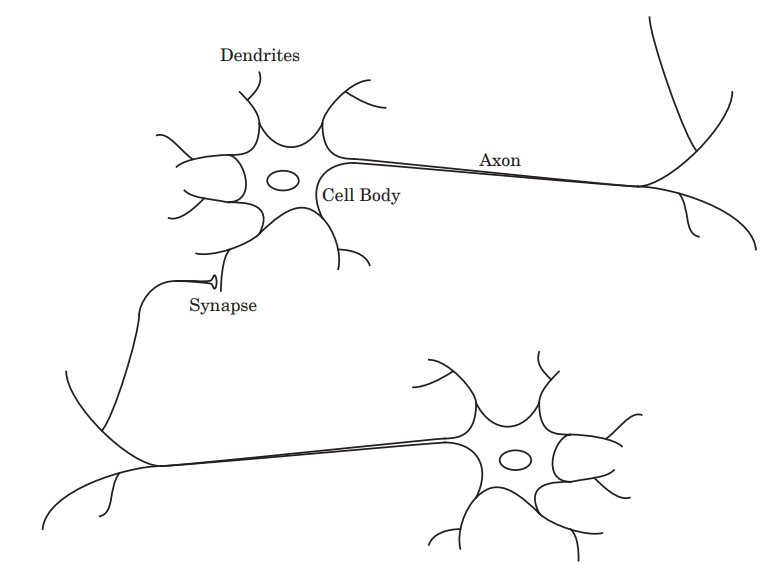
\includegraphics[width=\textwidth]{Neuronio}
%    Fonte: \citeonline{Neural_Network_Design}\hfill
%    \label{fig:figuraneuronio}
%\end{figure}

%As RNA's não tem a complexidade de células cerebrais, porém existem dois aspectos em que são semelhantes. O primeiro está relacionado aos elementos da rede que são meros dispositivos computacionais e são altamente interconectados, embora os neurônios artificias sejam muito mais simples. O segundo aspecto diz respeito as conexões entre os neurônios que determinam a função da rede. Embora neurônios biológicos sejam muito lentos em comparação com circuitos elétricos ($10^-3$ contra $10^-10$ s), nosso cérebro é capaz de realizar tarefas muito mais rápido que um computador devido à impressionante de estrutura de processamento paralelo existente nas redes neurais biológicas. 
%Nos dias atuais a Inteligência Artificial (IA) tem conseguindo resolver problemas que para os humanos são muito difíceis, problemas esses que são possíveis de serem declarados formalmente através de regras matemáticas, por outro lado as tarefas que se mostram desafiadoras para a IA são relativamente simples para os humanos mas são de difícil formalização, como o reconhecimento de palavras em um som ou particularidades em uma imagem. 
%As soluções que usam RNA permitem que computadores aprendam a partir de experiências e entendimento do mundo em termos de conceito de hierarquia, onde cada conceito é definido através de das suas relações com conceitos mais simples. Ganhando conhecimento através de experiências, RNA's não necessitam de um humano para formalmente especificar todo o conhecimento que %um computador necessita, as hierarquias permitem que os computadores aprendam conceitos complicados através de outros mais simples.

%%%%%%%

Neste trabalho as RNA serão utilizadas para detectar e segmentar objetos, que pertencentes a uma sequências de quadros como entrada. 


A seguir serão apresentado modelos matemáticos simplificados de neurônios artificiais, como formalizados por \citeonline{Neural_Network_Design} e como eles podem ser interconectados e dessa forma possam formar uma arquitetura de rede. 

A notação matemática utilizada utilizará será a seguinte:

\begin{itemize}
 
\item Escalar  — letras minúsculas em \textit{itálico}: \textit{a,b,c}
\item Vetores  — letras minúsculas em \textbf{negrito}: \textbf{a,b,c}
\item Matrizes — letras maiúsculas em \textbf{NEGRITO}: \textbf{A,B,C} 

\end{itemize}

\subsection {Neurônios de entrada única}

Um neurônio de entrada única pode ser visto na figura \ref{fig:Neurônio_geral1}, onde uma entrada escalar \textit{p} é multiplicada por um fator de ponderação \textit{w} formando assim \textit{wf} e enviado para a somatória. A outra entrada, de valor 1, é multiplicada por fator de erro \textit{b} e também enviado a somatória. O resultado da somatória é denominado como a entrada da rede e vai para uma função de transferência \textit{f} que produz um escalar \textit{a} como saída do neurônio,  representado pela equação \ref{eq:neuonio_simples}

\begin{figure}[H]
    \centering
    \caption{Neurônio de entrada única}
    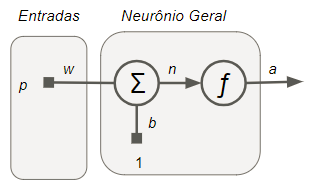
\includegraphics[scale=1]{Neuronio_geral1}\\
    Fonte: Autor\hfill
    \label{fig:Neurônio_geral1}
\end{figure}

  \begin{equation}
    a = {f(wp+b)}
    \label{eq:neuonio_simples}
  \end{equation}


 Os escalares \textit{w} e \textit{b} são parâmetros ajustáveis pela função de transferência que é escolhida pelo responsável pela rede neural, e com isso são ajustados por alguma regra de aprendizagem para que as relações de entrada e saída do neurônio atinjam alguma meta específica.
As funções de transferências são escolhidas para se satisfazer alguma especificação do problema que o neurônio está tentando resolver. A importância das funções de ativação é que elas trazem um componente não linear para as RNA, o que leva que seja possível que aprendam mais que relações lineares das variáveis, sejam elas dependentes ou independentes. As funções de ativação são responsáveis dentro da RNA por introduzir uma componente de não linearidade ao sistema, o que as diferenciam de um modelo de regressão linear. As três funções de ativação mais usadas serão apresentadas abaixo.

\begin{enumerate}
  \item Função Limiar\\
  A função Limiar, figura: \ref{fig:Hard_limit1}, define a saída do neurônio em 0 quando o resultado da função for menor que 0, ou 1 se seu argumento for maior ou igual a 0.
  
  \begin{figure}[H]
    \centering
    \caption{Função Limiar}
    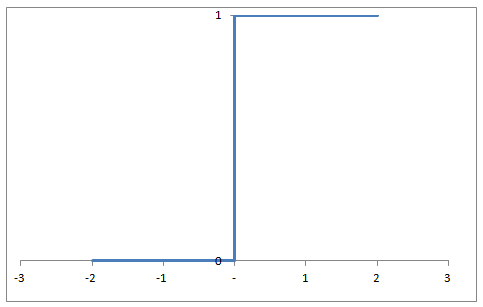
\includegraphics[scale=0.75]{Hard_limit1}\\
    Fonte: Autor\hfill
    \label{fig:Hard_limit1}
  \end{figure}
  
  
  \item Função Linear\\
  A saída da função linear é igual sua entrada, conforme mostra a figura \ref{fig:Linear}.
  
  \begin{figure}[H]
    \centering
    \caption{Função de transferência Linear}
    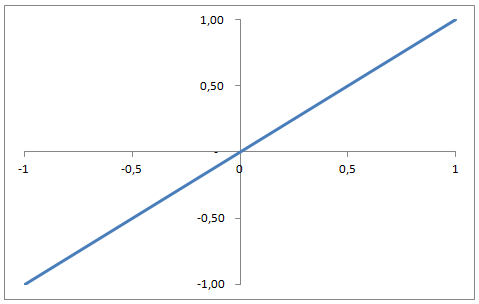
\includegraphics[scale=0.75]{Linear1}\\
    Fonte: Autor\hfill
    \label{fig:Linear}
  \end{figure}
  
  \item \textit{Função Log-sigmoide}\\
  A entrada para a função log-sigmoide, figura \ref{fig:Sigmoid}, varia de $\pm$  $\infty$ e limita a saída entre 0 e 1, de acordo com a equação \ref{eq:sigmoid}, este tipo de função é muito usada em redes com muitas camadas e que são treinadas usando algoritmos de retro propagação de erro, em especial porque esta função pode ser derivada.
  
  
  \begin{equation}
    a = \frac{1}{1+\textit{$e^\textit{-n}$}}
    \label{eq:sigmoid}
  \end{equation}
  
  \begin{figure}[H]
    \centering
    \caption{Função de transferência Sigmoide}
    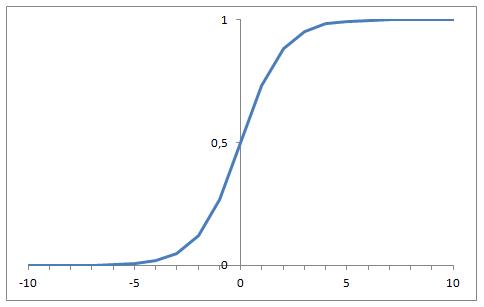
\includegraphics[scale=0.75]{Sigmoid}\\
    Fonte: Autor\hfill
    \label{fig:Sigmoid}
\end{figure}
  
\end{enumerate}


\subsection {Neurônios de múltiplas entradas}

Normalmente um neurônio tem mais de uma entrada, portanto um neurônio com \texttt{R} entradas, como na figura \ref{fig:Neuronio_multipla_entrada}, tem suas entradas individuais \textit{\(p_1, p_2,...,p_R \)}  ponderados pelos respectivos elementos \textit{\(w_1, w_2,...,w_R \)} da matriz do fator de ponderação \textbf{W}. O fator de erro é somado com as entradas já ponderadas para formar a entrada da rede \textit{n}, como visto na equação \ref{eq:m_entradas}: 

\begin{figure}[H]
    \centering
    \caption{Neurônio de múltiplas entradas}
    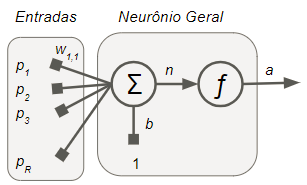
\includegraphics[scale=1]{Neuronio_multipla_entrada1}\\
    Fonte: Autor \hfill
    \label{fig:Neuronio_multipla_entrada}
\end{figure}

  \begin{equation}
    \textit{n} = \textit{\[w_{1,1}p_1 + w_{1,2}p_2 +...+ w_{1,R}p_R + b. \]}
    \label{eq:m_entradas}
  \end{equation}
  
  A equação \ref{eq:m_entradas} pode ser descrita na forma matricial, de acordo com a equação \ref{eq:multiplas_entradas1}:
  
 \begin{equation}
    \textit{n} = \textbf{Wp} + \textit{b}.
    \label{eq:multiplas_entradas1}
  \end{equation}
  
  Dessa maneira um neurônio pode ser definido de acordo com a equação \ref{eq:multiplas_entradas2}:
  
 \begin{equation}
    \textit{a} = \textit{f}(\textbf{Wp} + \textit{b}).
    \label{eq:multiplas_entradas2}
  \end{equation} 
  
\subsection {Neurônios de uma camada} 

Uma rede com apenas uma camada de neurônios S, como mostrado na figura \ref{fig:Neuronio_uma_camada}, recebe cada entrada \textbf{p} que está conectada com cada neurônio através da matriz do fator de ponderação, e recebe um fator de erro na somatória, que passa seu resultado para a função de transferência para gerar a saída \textit{a}.


\begin{figure}[H]
    \centering
    \caption{Rede com uma camada de neurônios}
    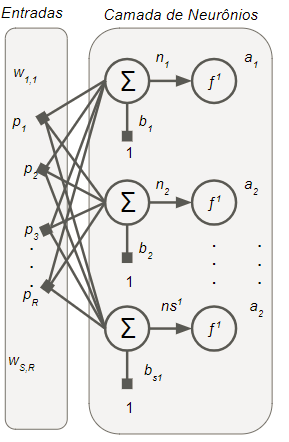
\includegraphics[scale=1]{Camada_neuronios1}\\
    Fonte: Autor\hfill
    \label{fig:Neuronio_uma_camada}
\end{figure}

A matriz do fator de ponderação \textbf{W} é representada pela equação \ref{eq:multiplas_entradas}:

 \begin{equation}
    \textit{a} = \textit{f}(\textbf{Wp} + \textit{b}).
    \label{eq:multiplas_entradas}
  \end{equation} 
  

Cada linha da matriz \textbf{W}, de acordo com a equação \ref{eq:matriz_pond} indica o neurônio destino à qual os fatores de ponderação estão associados, enquanto as colunas indicam a fonte da entrada de cada fator de ponderação.

\begin{equation}
\centering
\textbf{W} ={\begin{bmatrix}
    w_{1,1} & w_{1,2} & \cdots & w_{1,R}\\
    w_{2,1} & w_{2,2} & \cdots & w_{2,R}\\
    \vdots & \vdots & \ddots & \vdots \\
    w_{S,1} & w_{S,2} & \cdots & w_{S,R}
\end{bmatrix}}
\label{eq:matriz_pond}
\end{equation} 

\subsection {Neurônios de múltiplas camadas} 

Em uma rede com vários neurônios, como visto na figura \ref{fig:Neuronio_multipla_camada}, cada camada tem sua própria matriz de ponderação \textbf{W}, seus próprios vetores de fator de erro \textbf{b} e de entrada \textit{n} e uma saída \textbf{a}. Para definir todos esses elementos de cada camada, um índice sobrescrito foi incluído em cada termo. Uma camada onde a saída é a própria saída da rede é chamado de \textit{camada de saída} todas as outras camadas são denominadas \textit{camadas ocultas}. 
Redes Neurais multicamadas tem mais capacidade de resolver problemas que as redes simples, como exemplo uma rede de duas camadas tendo uma \textit{log-sigmoide} na primeira camada e uma linear na segunda pode ser treinada para aproximar funções, porém as de camada única não. 

\begin{figure}[H]
    \centering
    \caption{Rede com múltiplas camadas de neurônios}
    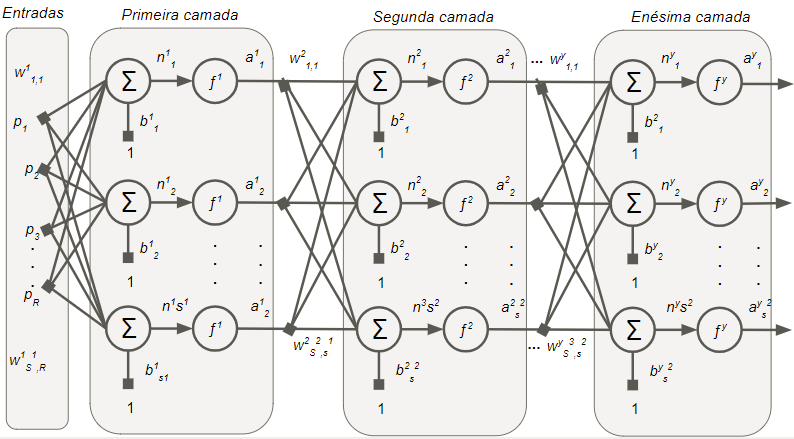
\includegraphics[scale=0.65]{neuronio_multi_camada1}\\
    Fonte: Autor\hfill
    \label{fig:Neuronio_multipla_camada}
\end{figure}

\subsection {Redes recorrentes}

As redes neurais recorrentes são redes com realimentação de informações da saída diretamente para a matriz \textbf{W}, ou seja suas saídas estão conectadas as entradas, um exemplo de rede recorrente discreta em relação ao tempo pode ser vista na figura \ref{fig:rederecorrente}. Redes recorrentes são poderosas se comparadas com as não recorrentes em especial pelo motivo de as saídas futuras serem computadas levando-se em conta as saídas de períodos anteriores.

\begin{figure}[H]
    \centering
    \caption{Rede recorrente}
    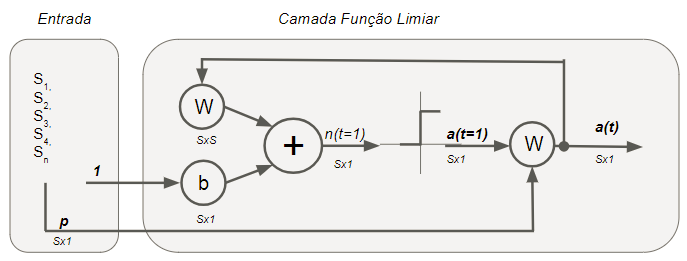
\includegraphics[scale=0.75]{Rede_recorrente1}\\
    Fonte: Autor\hfill
    \label{fig:rederecorrente}
\end{figure}


\subsection{Redes neurais de alimentação direta}

As técnicas modernas utilizada em aprendizado de máquina são uma estrutura poderosa para o aprendizado supervisionado de acordo com \citeonline{Goodfellow-et-al-2016}. Uma RNA pode aumentar sua complexidade adicionando-se mais camadas ou mesmo mais entradas em cada camada. 

Nesta seção será apresentado segundo \citeonline{Neural_Network_Design} o modelo básico de uma RNA, chamado de Perceptron. 

%e as RNC's que são atualmente utilizadas para atividades de reconhecimento e detecção de objetos em imagens.%

Perceptrons ou Redes Neurais de alimentação direta, como mostrado na figura \ref{fig:perceptron},  tem sua saída definida pela equação \ref{eq:perceptron}:

 \begin{equation}
    \textbf{a  = Limiar(Wp+b)}.
    \label{eq:perceptron}
  \end{equation} 
  
\begin{figure}[H]
    \centering
    \caption{Perceptron}
    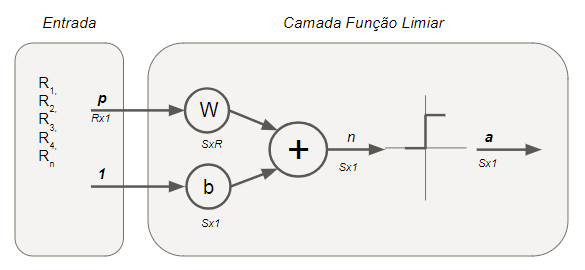
\includegraphics[scale=1]{perceptron1}\\
    Fonte: Autor\hfill
    \label{fig:perceptron}
\end{figure}

Considerando a seguinte matriz de ponderação da equação \ref{eq:matrix} :

\begin{equation}
\centering
\textbf{W} ={\begin{bmatrix}
    w_{1,1} & w_{1,2} & \cdots & w_{1,R}\\
    w_{2,1} & w_{2,2} & \cdots & w_{2,R}\\
    \vdots & \vdots & \ddots & \vdots \\
    w_{S,1} & w_{S,2} & \cdots & w_{S,R}
\end{bmatrix}}
\label{eq:matrix}
\end{equation} 

Consideraremos um vetor composto o enésimo elemento da coluna de \textbf{W}, conforme equação \ref{eq:vetor}:

\begin{equation}
\centering
\textbf{$_i$W} ={\begin{bmatrix}
    w_{i,1}\\
    w_{i,2}\\
    \vdots \\
    w_{i,R}
\end{bmatrix}}
\label{eq:vetor}
\end{equation}

Então é possível particionar o vetor de ponderação conforme a equação \ref{eq:vetor_ponderacao}:

\begin{equation}
\centering
\textbf{$_i$W} ={\begin{bmatrix}
    \textbf{$_1$W}^T\\
    \textbf{$_2$W}^T\\
    \vdots \\
    \textbf{$_S$W}^T
\end{bmatrix}}
\label{eq:vetor_ponderacao}
\end{equation}

A partir dessas equações podemos escrever o enésimo elemento do vetor de saída da rede como mostrado na equação \ref{eq:vetor-saida} :

\begin{equation}
\centering
    a_1=\textit{Limiar}(\textbf{$_i$W}^T\textbf{p}+\textit{$b_i$}).
    \label{eq:vetor-saida}
\end{equation}

As redes neurais de alimentação direta tem sua saída computada diretamente em uma única passada pela rede, não existe retro alimentação. Este tipo de estrutura é comumente utilizada para reconhecimento de padrões, para aproximação de funções que serão usadas em filtros adaptativos e também em controles automáticos.

Na próxima seção será apresentado um caso especial de redes neurais de alimentação direta, chamadas de redes neurais convolucionais. As redes neurais convolucionais atualmente, como mostrado no capítulo 2, tem se mostrado eficiente para o processamento de imagens quando é necessário detectar e classificar objetos em uma imagem.


\subsection{Redes Neurais Convolucionais}
As RNC são um tipo especial das redes neurais de alimentação direta de acordo com  \citeonline{Goodfellow-et-al-2016}, são simplesmente redes neurais que utilizam convolução ao invés de multiplicação de matrizes em pelo menos uma de suas camadas, são utilizadas principalmente para processamento de dados com topologia do tipo grade, como imagens por exemplo que tem duas dimensões.. As redes convolucionais obtiveram bastante exito em em aplicações práticas, principalmente com imagens. 
O nome convolução é operação matemática linear entre duas funções com valores reais e definido na equação \ref{eq:convolucao}:

\begin{equation}
\centering
    \textit{s(t)=(x \textasteriskcentered w )(t)}.
    \label{eq:convolucao}
\end{equation}

O argumento \textit{w} da função \ref{eq:convolucao} deve ser uma função válida de probabilidade densa senão a saída não será uma média ponderada, deve também ser 0 para todos argumentos negativos. A função \textit{x} da equação \ref{eq:convolucao} é a entrada e \textit{w} o kernel, sua saída é denominada de mapa de característica. No caso de imagens, o tempo é discreto, portanto podemos assumir que \textit{t} é um valor inteiro e que tanto \textit{x} quanto \textit{w} estão restritos ao inteiro \textit{t}, com isso é possível definir uma convolução discreta na equação \ref{eq:convolucao1}

\begin{equation}
\centering
    \textit{s(t)=(x \textasteriskcentered w )(t)} = \sum_{a=- \infty}^{\infty} \textit{(a)w(t-a)} .
    \label{eq:convolucao1}
\end{equation}

Para imagens, utilizamos convolução em mais de um eixo por vez, neste caso utilizamos um kernel de duas dimensões, como mostrado na equação \ref{eq:convolucao2}:


\begin{equation}
\centering
    \textit{s(i,j)=(K\textasteriskcenteredI I)((i,j))} = \sum_{m} \sum_{n} \textit{I(m,n)K(i-m, j-n)} .
    \label{eq:convolucao2}
\end{equation}

Uma convolução é comutativa, por isso pode ser definida também como visto na figura \ref{eq:convolucao3}:

\begin{equation}
\centering
    \textit{s(i,j)=(I\textasteriskcenteredI K)((i,j))} = \sum_{m} \sum_{n} \textit{I(i-m, j-n)K(m,n)} .
    \label{eq:convolucao3}
\end{equation}


No exemplo da figura \ref{fig:convolução} uma imagem binária de 5x5 utilizada como entrada I para a convolução e um kernel K 3x3 tem o resultado no mapa de característica de convolução o valor 2 como pode ser visto na soma dos produtos I por K.

\begin{figure}[H]
    \centering
    \caption{Exemplo convolução}
    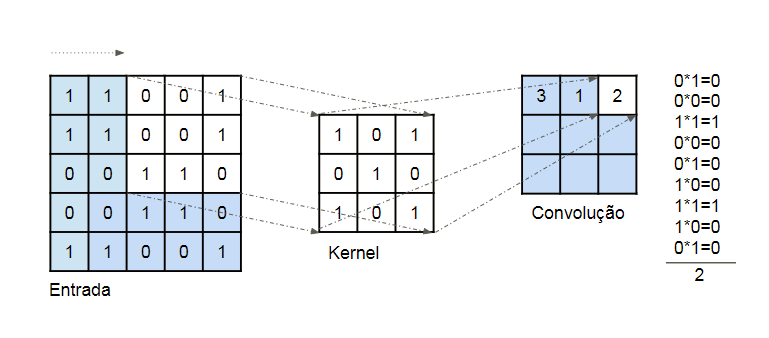
\includegraphics[scale=0.65]{convolucao1}\\
    Fonte: Autor\hfill
    \label{fig:convolução}
\end{figure}

A convolução traz 3 importantes ideias com ajudam a melhorar o sistema de aprendizado de máquina:

\begin{itemize}
    \item Interações esparsas: Em RNA tradicionais se multiplicam uma matriz por outra matriz, isso significa que toda saída sempre interage com toda entrada enquanto nas RNC utilizamos um kernel muito menor que o tamanho da entrada, isso significa uma redução grande de memória e que a computação da saída requer menos operações. No exemplo da figura \ref{fig:esparso}, uma entrada \textit{$x_3$} e as saídas \textit{s}, que estão em destaque, mostram que utilizando um kernel de tamanho 3, apenas 3 saídas são impactadas por \textit{x} (superior). Por outro lado quando a saída \textit{s} é resultado de uma multiplicação de matrizes a conectividade não é mais esparsa e portanto todas as saídas são afetadas por uma única entrada \textit{$x_3$} (inferior).
    
\begin{figure}[H]
    \centering
    \caption{Conectividade esparsa}
    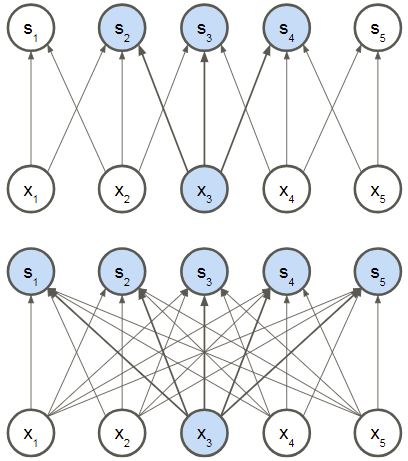
\includegraphics[scale=1]{esparso1}\\
    Fonte: Autor\hfill
    \label{fig:esparso}
\end{figure}
    
        \item Compartilhamento de parâmetros: Cada membro do kernel é utilizado em todas as posições dos dados de entrada, e faz com que ao invés de aprender parâmetros separados para cada posição, é aprendido apenas um conjunto. De fato isso não afeta o tempo de processamento da propagação direta, porém reduz muito a necessidade de memória para um modelo que utiliza, por exemplo, valores de kernel k de 3x3, 5x5, e 7x7 se comparado com as dimensões de uma imagem inteira. A figura \ref{fig:compartilhamento} mostra as conexões em setas em negrito, na parte superior, indica o uso de kernel de 3 elementos em um modelo convolucional. Na parte de baixo indica o uso de uma matriz ponderada totalmente conectada. RNA's que utilizam esse método, cada entrada tem sua própria matriz de ponderação, ou seja neste caso não há compartilhamento de parâmetros como o kernel compartilha em redes convolucionais.
 
\begin{figure}[H]
    \centering
    \caption{Compartilhamento de parâmetros}
    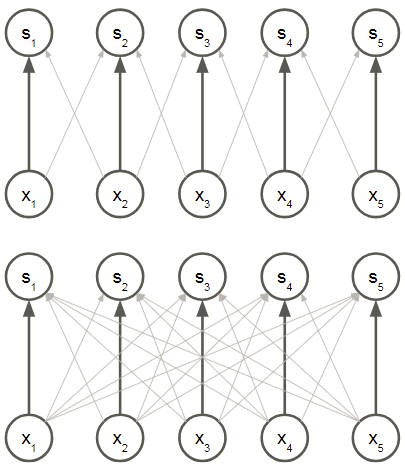
\includegraphics[scale=1]{compartilhamento1}\\
    Fonte: Autor\hfill
    \label{fig:compartilhamento}
\end{figure}       
        
        
    \item Representações Equivariantes: A forma particular com que as convoluções compartilham parâmetros faz com que a camada tenha uma propriedade equivariante em relação a translação da entrada, independente de onde o objeto está em uma imagem a capacidade de identificar suas bordas, será a mesma.
    
\end{itemize}

Uma típica camada de uma RNC tem três estágios, no primeiro estágio as camadas realizam várias convoluções em paralelo para produzir um conjunto de ativações lineares. No segundo estágio cada ativação linear é processada por uma função de ativação não linear, para RNC's a mais utilizada é a função de ativação linear retificada (ReLu). A figura \ref{fig:relu} mostra o gráfico da função $f(x)=max(0,x)$, que tem saída 0 sempre que a entrada for menor que zero, e tem saída igual à entrada para todos os valores maiores que 0.  

\begin{figure}[H]
    \centering
    \caption{Função ReLu}
    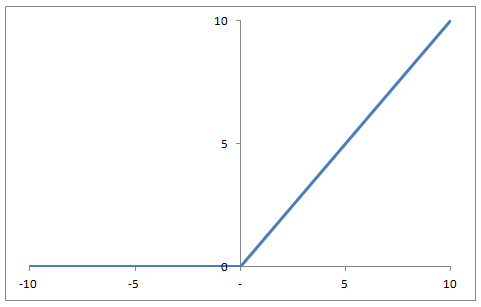
\includegraphics[scale=0.75]{ReLu}\\
    Fonte: Autor\hfill
    \label{fig:relu}
\end{figure} 

No terceiro estágio tem-se uma camada com a função de agregação que modifica a saída da camada, esta função substitui a saída da rede em certas regiões com uma síntese estatística das saídas próximas. É comum inserir camadas de agregação entre camadas sucessivas de convolução pois ela reduz o tamanho espacial da representação do problema para reduzir a quantidade de parâmetros e computação na rede. A forma mais comum de agregação é uma filtragem de tamanho 2x2 com passo 2, este processo reduz em 75$\%$ o tamanho do problema. Na figura \ref{fig:pooling}, pode-se checar que a função de agregação reduz o tamanho espacial do problema, o tamanho da entrada é 300x300x64, e utilizando-se uma função de agregação com filtro tamanho 2x2 e com passo 2 o tamanho é reduzido para 150x150x64. A operação mais comum para função de agregação é o máximo valor, que copia o máximo valor da dentro do filtro de 2x2 como mostrado no exemplo.


\begin{figure}[H]
    \centering
    \caption{Função de agregação}
    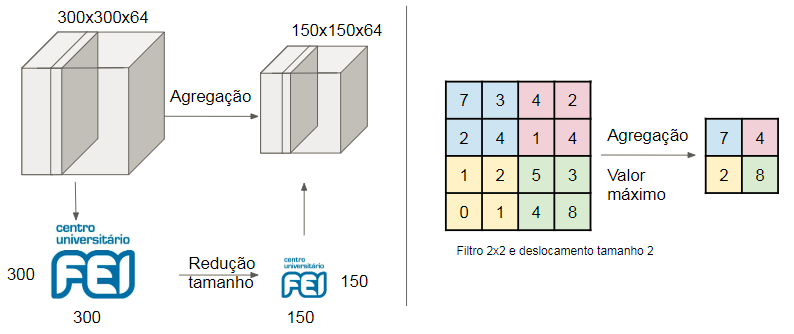
\includegraphics[width=\textwidth]{pooling1}\\
    Fonte: Autor\hfill
    \label{fig:pooling}
\end{figure} 


A forma mais comum de arquitetura de uma RNA é combinação de algumas camadas de convolução com função de ativação ReLu seguidas por camadas de agregação, como pode ser visto na figura \ref{fig:camada_convolucao}, e repetem esse padrão até que a imagem possa ser fundida espacialmente a um pequeno tamanho. A última camada é totalmente conectada e corresponde à saída da RNC, representado pela figura \ref{fig:RNC}.

\begin{figure}[H]
    \centering
    \caption{Camada de convolução}
    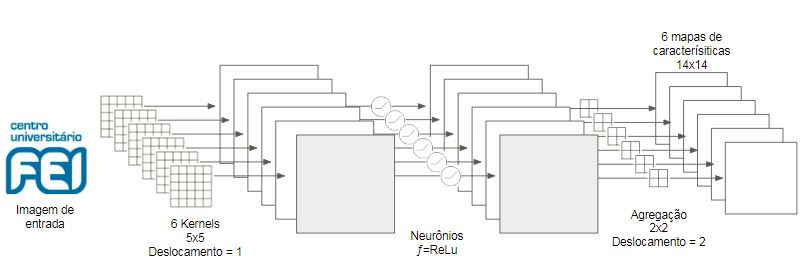
\includegraphics[width=\textwidth]{camada_convolucao1}\\
    Fonte: Autor\hfill
    \label{fig:camada_convolucao}
\end{figure} 

\begin{figure}[H]
    \centering
    \caption{Rede Neural Convolucional}
    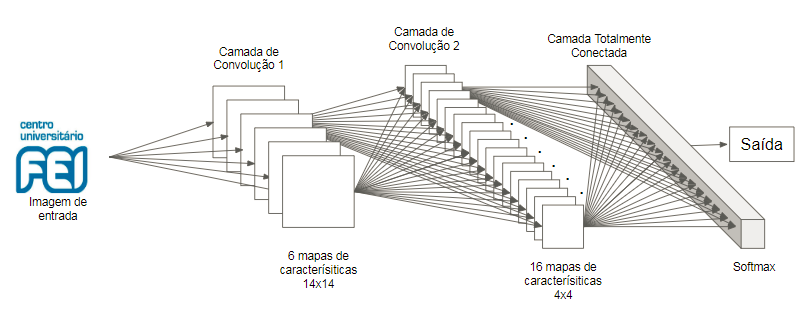
\includegraphics[width=\textwidth]{RNC1}\\
    Fonte: Autor\hfill
    \label{fig:RNC}
\end{figure} 




Uma RNC pode ser usada para gerar na sua saída um objeto estruturado de grande dimensão, ao invés de apenas de fazer a predição de uma classe para tarefas de classificação ou mesmo um valor real para uma atividade de regressão. Normalmente a saída é um tensor \textbf{S}, onde \textbf{$S_{i,j,k}$} é a probabilidade que cada pixel (\textit{j,k}) de uma entrada pertencer a uma classe \textit{i}. Isso permite que o modelo classifique cada pixel em uma imagem e crie uma mascara que permite acompanhar os contornos dos objetos.

%%% deletar a seção 3.1.8 (toda ela). Tb está fora de contexto %%%

%\subsection{Regras de aprendizado}

%As regras de aprendizado, em geral são procedimentos que alteram os valores dos fatores de ponderação e erro de uma RNA, esses procedimentos também são chamados de treinamento. Existem três grandes categorias de aprendizado:

%\begin{itemize}
%    \item Aprendizado supervisionado: Neste tipo de aprendizado é fornecido uma série de exemplos para as redes com o comportamento que se espera da própria rede, como mostrado na equação \ref{eq:aprendizadosupervisionado}, onde \textbf{$p_q$} é uma entrada da rede e \textbf{$t_q$} é sua correspondente saída correta. Conforme as entradas são aplicadas na entrada da rede as saídas são comparadas com o objetivo, o aprendizado então é utilizado para ajustar os fatores de ponderação e erro com o objetivo de fazer com que as saídas fiquem o mais perto possível do objetivo.
    
%    \begin{equation}
%         \textbf{\[ \left \{ p_1, t_1 \right \}, \left \{ p_2, t_2 \right \}, ..., \left \{ p_Q, t_Q \right \} \]}
%         \label{eq:aprendizadosupervisionado}
%    \end{equation}
    
%    Segundo \citeonline{Goodfellow-et-al-2016}, os principais métodos de aprendizado supervisionado são os algoritmos que estimam a distribuição das probabilidades p(t|\textbf{p}) através da estimação da máxima semelhança, regressão linear e máquinas de vetor de suporte entre outros citados.
    
%    \item Aprendizado por reforço: É similar ao aprendizado supervisionado, porém ao invés de utilizar uma saída correta para para cada entrada da rede, o algoritmo apenas devolve uma nota, e esta nota é a performance da rede quando submetidas a uma sequência de entradas. Atualmente este tipo de solução é pouco utilizada de acordo com \citeonline{Neural_Network_Design} .
    
%    \item Aprendizado não supervisionado: Os pesos e os erros são modificados de acordo apenas com as entradas da rede, não existe um valor de saída disponível, os algoritmos de aprendizado não supervisionado segundo \citeonline{Goodfellow-et-al-2016} agrupam as entradas através de exemplos similares e também através da distribuição de probabilidades da base de dados.
    
%\end{itemize}




%%----------------------%%

% Assuntos on Hold

%%\subsubsection {Redes recorrentes}

%%\subsubsection{Redes Neurais de Hamming}

%%\subsubsection{Redes Neurais de Hopfield}

%%-----------------------%%


%% Fator de ponderação = weight // Fator de erro = bias

\newpage
\section {Programação em Lógica}
 O modelamento e o raciocínio sobre dados relacionais, como explicado em \citeonline{10.1007/978-3-319-23461-8_37} pode ser feito através de uma paradigma de programação, a Programação em Lógica (PL). Programas lógicos são uma coletânea de afirmações que são verdadeira dado um domínio. Apesar de muitas aplicações aprendizado de máquina utilizarem-se de ferramentas de PL, a necessidade de raciocínio mais eficiente para tratar incertezas levou ao desenvolvimento de formalismo como a Programação em Lógica Probabilística (PLP). PLP vai além da lógica pura onde uma afirmação deve ser verdadeira ou falsa, e considera que uma afirmação pode ser incerta e determina uma probabilidade a ela.


\subsection{ProbLog}

De acordo com \citeonline{10.1007/978-3-319-23461-8_37}, \textit{ProbLog} é o estado da arte da implementação de uma linguagem de programação em lógica probabilística, seu objetivo comum é disponibilizar uma ferramenta poderosa para modelamento e raciocínio de sobre domínios estruturado e domínios incertos que aparecem em aplicações como em reconhecimento de atividades, processamento de linguagem natural, etc. O desenvolvimento do \textit{ProbLog} foi focado especialmente para ser utilizado em técnicas de aprendizado de máquina e sua implementação, além disso é a única linguagem de programação que possibilita por exemplo, múltiplas consultas durante o cálculo das probabilidades marginais, além de poder incorporar novas evidências.

\citeonline{10.1007/978-3-319-23461-8_37} explica que \textit{ProbLog} é uma ferramenta que consiste na linguagem de programação \textit{ProbLog} também na inferência e aprendizagem em \textit{ProbLog}. Inicialmente \textit{ProbLog} fo proposto como uma ferramenta de PLP com o objetivo principal de calcular a probabilidade de sucesso de uma pesquisa, comumente este sistema foi chamado de \textit{ProbLog1}. A evolução do \textit{ProbLog} para um linguagem capaz de representar modelos gráficos através de lógica e representações relacionais com por exemplo, os modelos probabilísticos relacionais e programas lógicos Bayesianos, é chamado de \textit{ProbLog2}. 

\subsubsection{Sintaxe}
ProbLog, como demonstrado em \citeonline{phdthesis_ProbLog}, é uma linguagem de Programação em Lógica Probabilística (PLP) de propósito geral, os fatos probabilísticos podem ser simples ou compostos por mais de uma variável. Os fatos probabilísticos são as mais básicas estruturas para representar a incerteza dos dados.

A representação de um fato probabilístico tem a forma $p_{i}$ :: $f_{i}$ e afirma que que o fato $f_{i}$ é verdade com probabilidade $p_{i}$ ou falso com probabilidade $(1-p_{i})$. As regras em ProbLog definem consequências lógicas de fatos probabilísticos. 

No exemplo da figura \ref{fig:graph_acyclic} um grafo modela a incerteza entre duas entidades, que são representadas por nós e cada dependência é uma ligação com sua respectiva probabilidade.


\begin{figure}[H]
    \centering
    \caption{Grafo acíclico de 3 nós}
    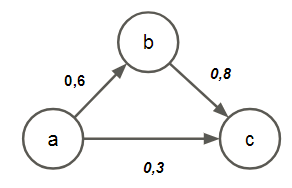
\includegraphics[scale=1.3]{graph_acyclic1}\\
    Fonte: Autor\hfill
    \label{fig:graph_acyclic}
\end{figure} 

Em ProbLog, o grafo da figura \ref{fig:graph_acyclic} é representado da seguinte maneira:

$0.6::e(a, b).  $ $0.3::e(a, c).  $ $0.8::e(b, c).$ \newline

$p(X, Y) :- e(X, Y). $ \newline

$p(X, Y) :- e(X, X1), p(X1, Y). $ \newline

O fato $0.6::e(a, b)$ expressa uma ligação existente ente os nós $a$ e $b$ com probabilidade de $0.6$. Todos os possíveis nós de um grafo são representados dessa maneira, nós que não existirem podem ser omitidos ou serem declarados como probabilidade zero, por exemplo: um nó de $b$ para $a$ seria expresso da seguinte modo $0.0::e(b, a)$.

Um átomo que se unifica com fato probabilístico é chamado de \textit{átomo probabilístico} e um átomo que se unifica com a cabeça de uma regra é chamado de \textit{átomo derivado}. Um conjunto de átomos derivados e átomos probabilísticos de um programa em ProbLog é uma disjunção. Tomando a figura \ref{fig:graph_acyclic} como exemplo temos:

\{$e(a, b), e(a, c), e(b, c)$\}.\newline

\{$p(a, b), p(a, c), p(b, c), P(a, c)$\}.\newline

Além dos fatos probabilísticos a linguagem utilizado pelo sistema \textit{ProbLog2}, também suporta fatos probabilísticos intencionais, que são utilizados para compactar um conjunto de fatos probabilísticos, a seguinte forma é utilizada: $P :: f(X_1,...,X_n):- Corpo.$, onde o corpo é a conjunção de literais e não incluem outros fatos probabilísticos. a probabilidade $P$ pode ser um número ou ainda uma variável que unifica com um número quando o corpo é provado, as variáveis $X_1$ até $X_n$ são instanciadas quando o corpo é provado.

No seguinte fato probabilístico intencional:

$0.3::(A, B) :- membro(A, [a, b]), membro(B, [c,d])$

Estão compactados a representação dos seguintes fatos:

$0.3::nó(a, c)$

$0.3::nó(a, d)$

$0.3::nó(b, c)$

$0.3::nó(a, d)$


\subsubsection{Semântica}

Todo fato probabilístico de um programa de \textit{ProbLog} é um variável aleatória binária e que pode ser verdadeiro ou falso, além disso a escolha do valor verdade de uma átomo probabilístico é chamado de \textit{escolha atômica}, a escolha atômica de todas as probabilidades é a \textit{escolha total}. Para \textit{n} fatos probabilísticos, existem $2^n$ escolhas totais e cada escolha forma um único modelo de programa em ProbLog e é chamado de \textit{mundos possíveis}. Dado que átomos probabilísticos são considerados variáveis independentes e randômicas, é possível determinar a probabilidade de um possível mundo, como o produto das probabilidades associadas com as escolhas atômicas. 

Sendo $Ω = {ω_1, .., ω_N }$ um conjunto de mundos possíveis em um programa escrito em ProbLog, onde $N=2^n$, sendo que $n$ é o número de átomos probabilísticos. Uma vez que apenas átomos probabilísticos tenham probabilidades, um  único mundo possível pode ser mostrado como uma tupla $(w_i^+, w_i^-)$, onde $w_i^+$ é o conjunto de átomos probabilísticos em $w_i$ que são verdadeiros e $w_i^-$ são falsos.

Formalmente, um programa em ProbLog define a distribuição sobre todos os possíveis mundos como mostrado na equação \ref{eq:distribuição_possiveis_mundos}, onde $p_i$ são as probabilidades dos átomos $a_i$.

\begin{equation}
\centering
    P(w_i)= \prod_{a_j\in w_i^+} p_j \prod_{a_j\in w_i^-} (1-p_j)
    \label{eq:distribuição_possiveis_mundos}
\end{equation}


A somatória sobre as probabilidades de todos os possíveis mundos em programa em \textit{ProbLog} é igual a um, conforme a equação \ref{eq:distribuição_possiveis_mundos}: 

\begin{equation}
\centering
    \sum_{w_i \in \Omega } {P(w_i)=1}
    \label{eq:distribuição_possiveis_mundos}
\end{equation}

Uma pesquisa de um átomo $q$ é verdadeira em todos os possíveis mundos $w^q$ se o modelo expresso pelo mundo implica $q$ ($w^q \models q$).

A pesquisa $p(a, c)$ realizada para o grafo da figura \ref{fig:graph_acyclic} é verdadeira se se existir pelo menos um caminho entre os nós $a$ e $c$. Esta pesquisa é verdadeira em 5 dos possíveis $2^3=8$ possíveis mundos, como pode ser visto tabela \ref{tab: possiveis mundos} abaixo:

            \begin{table}[H]
                \centering % used for centering table
                \caption{Possíveis mundos entre $a$ e $c$}
                \begin{tabular}{c c c c c } % centered columns (2 columns)
                \hline\hline %inserts double horizontal lines
                Mundos possíveis & $nó(a,b)$ & $nó(a,c)$ & $nó(b,c)$ & Probabilidades\\  % inserts table
                %heading
                \hline  % inserts single horizontal line
                $w_1$ & T 0.6 & T 0.3 & T 0.8 & \textbf{0.144}\\
                $w_2$ & T 0.6 & T 0.3 & F 0.2 & \textbf{0.036}\\
                $w_3$ & T 0.6 & F 0.7 & T 0.8 & \textbf{0.336} \\
                $w_4$ & T 0.6 & F 0.7 & F 0.2 & 0.084 \\
                $w_5$ & F 0.4 & T 0.3 & T 0.8 & \textbf{0.096} \\ 
                $w_6$ & F 0.4 & T 0.3 & F 0.2 & \textbf{0.024} \\
                $w_7$ & F 0.4 & F 0.7 & T 0.8 & 0.224 \\
                $w_8$ & F 0.4 & F 0.7 & F 0.2 & 0.056\\
                      &       &       & \sum =& 1.000  \\        [0.5ex] 
                
                \end{tabular}
                \label{tab: possiveis mundos}
            \end{table}
            



\subsubsection{Inferência e aprendizado}

A linguagem \textit{ProbLog} realiza os seguintes tipos de inferência:

\begin{itemize}
    \item Probabilidade Marginal: Sendo $L$ um programa em \textit{ProbLog} e um conjunto de átomos probabilísticos $At$ e uma pergunta $Q \subseteq At$, é soma de todas as probabilidades onde a pergunta $q \in Q$ é verdade para um programa em \textit{ProbLog} $L: P(q)$. No exemplo da tabela \ref{tab: possiveis mundos} é a soma das probabilidades que estão em negrito, $p(a, c)=0,636$.
    
    \item Probabilidade Condicional: É o calculo da probabilidade dados as evidências observadas. Evidências é um conjunto de tuplas de átomos e seus respectivos valores verdades observados, formalmente uma evidência é $E=e$ onde $E \subset At$ é o conjunto de átomos e $e$ é o conjuto de valores verdade. A probabilidade condicional de uma pesquisa $q \in Q$ é o cálculo da relação \(P(q|E=e)=\frac{P(q\wedge E=e)}{P(E=e)}\). No exemplo do grafo acíclico da tabela \ref{tab: possiveis mundos} para a pesquisa $p(a,c)$ dado como evidência que o $nó(a,c)=falso$, temos: $P(p(a, c)|e(a, c) = false) =0.48$ 
    
    \item Máximo a Posteriori: Além do máximo a posteriori, calcula também seu caso especial: Explicação mais provável. Dado um programa $L$ em \textit{ProbLog} e um conjunto de átomos $At$, uma pesquisa $Q$ e evidências &E=e& em que $\{Q \cup E\}\subset At$, o cálculo de Máximo a Posteriori é encontrar os átomos probabilísticos mais prováveis para cada átomo probabilístico da pesquisa onde as evidências estão no estado determinado na pesquisa. No cálculo da explicação mais provável, o valor máximo de $argmax_\textbf{p}P(Q=q|E=e)$ onde $\textbf{q}$ é um conjunto dos valores verdade para cada $q\in Q$. No exemplo do grafo acíclico da tabela \ref{tab: possiveis mundos}, dada a evidência $nó(a,b)= falso$ o estado que demostra a explicação mais provável é $w7$ com $P=0,224$, pois tem a maior probabilidade dentre todas os possíveis mundo dado que $nó(a,b)= falso$.
    
\end{itemize} 

Programas em \textit{Problog} podem aprender parâmetros dado parciais interpretações do próprio programa. Uma interpretação parcial é um conjunto de átomos com seus respectivos valores observados. Para um dado programa em \textit{ProbLog} que contenha um conjunto de fatos probabilísticos com valores das probabilidades desconhecidos, a tarefa de aprendizado através de interpretações, calcula as probabilidades através do método de explicação mais provável dos fatos probabilísticos dado as evidência de alguns átomos. Este tipo de aprendizagem também utiliza inferência condicional para atualizar as probabilidades dos fatos probabilísticos iniciais até que exista convergência.

Neste capítulo foram apresentadas as teorias de Redes Neurais e Lógica Probabilística que serão necessárias para a base da proposta deste trabalho. No próximo capítulo será apresentada a proposta deste trabalho, e mostrará com mais profundidade como serão utilizadas as Redes Neurais e a Lógica probabilística como ferramentas para a criação de um sistema de auxílio ao motorista, com o objetivo de classificar automaticamente o risco de colisão entre automóveis.


%\subsubsection{Funções do programa}


%%%%%


%---parei!!!%

% --- Seção dentro do capítulo



\chapter {Proposta}

\section {Objetivo}
O objetivo deste trabalho é desenvolver um sistema de assistência ao motorista capaz de classificar automaticamente o risco de colisão durante ultrapassagens em tráfego de veículos, de acordo com o Código Brasileiro de Trânsito. Utilizando-se RNC para analisar uma sequência de quadros captados por uma câmera acoplada a um veículo, a RNC deverá segmentar e classificar, veículos, sinalizações de solo e placas de sinalização dentro de um contexto de tráfego de veículos, a fim de gerar na sua saída um vetor com esses dados, que será utilizado como evidências para um sistema de inferência lógico probabilístico, escrito na linguagem probabilística \textit{ProbLog}. Este sistema de inferência lógico probabilístico também receberá informações de uma base de conhecimento que conterá regras do ultrapassagens previstas no Código Brasileiro de Trânsito. O sistema realizará inferência do risco de colisão desse contexto específico, com o objetivo de gerar um alerta quando o risco inferido for relevante.

\section {Justificativa}
Os sistemas avançados de assistência ao motorista (ADAS) vem crescendo nos últimos anos, por duas razões. A primeira é regulatória, nos Estados Unidos e nos países da União Europeia já será obrigatório que em 2020 existam sistemas  de freio de emergência e sistemas de alertas de colisão. A segunda é mercadológica, motoristas estão cada vez mais interessados em carros com esses sistemas de assistência. Atualmente a Euro NCAP, entidade criado pelo Reino Unido e financiada pela União Europeia, e que realiza testes destrutivos em automóveis com o objetivo de avaliar a segurança dos ocupantes, através de um protocolo bem rígido de testes, somente dá nota máxima para veículos que atualmente já possuem sistemas de freio automático que previnam colisão ou que as amenize em caso extremos. A Euro NCAP em suas pesquisas identificou que motoristas, por desatenção ou erro, tem o tempo de reação de frear atrasadas em relação ao tempo necessário para se evitar a colisão. Para atender essa demanda, este trabalho pretende desenvolver um sistemas de assistência ao motorista que se utiliza de RNC em conjunto com um sistema lógico probabilístico para classificação de situações de risco em contextos de tráfego de veículos.

\section {Método}

O sistema proposto no trabalho é esquematizado na figura \ref{fig:diagrama_de_blocos}.

\begin{figure}[H]
    \centering
    \caption{Diagrama de blocos do sistema proposto}
    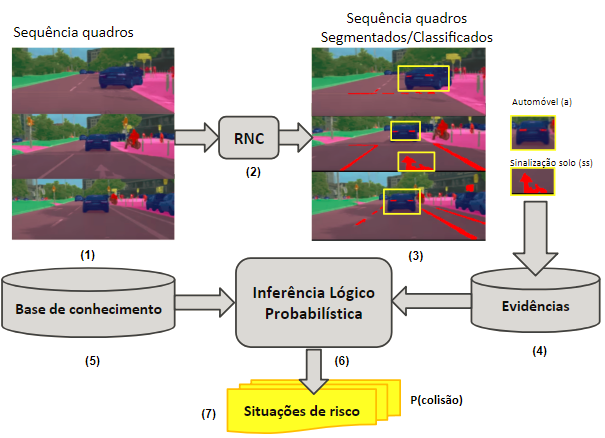
\includegraphics[width=\textwidth]{diagrama_de_blocos_v6}\\
    Fonte: Autor\hfill
    \label{fig:diagrama_de_blocos}
\end{figure} 

O funcionamento de cada etapa enumerada na figura \ref{fig:diagrama_de_blocos}, é apresentada abaixo, onde os números de cada item referem-se ao números dos módulos da figura \ref{fig:diagrama_de_blocos}.

\begin{enumerate}
    

    \item[{(1)}] Uma sequência de quadros de uma situação de tráfego de veículos será usada como entrada para para ser analisada pelo sistema.


    \item[{(2)}] Uma RNC receberá na sua entrada a sequência de quadros do item (1), o segmentará e classificará informações de sinalização de solo, placas de sinalização e veículos como mostrado na figura \ref{fig:diagrama_de_blocos}.


    \item[{(3)}] A saída da RNC conterá as informações segmentadas e classificadas com a probabilidades dos objetos detectados estarem na cena, no exemplo da figura \ref{fig:diagrama_de_blocos}, temos:
        \begin{itemize}
            \item Automóvel.
            \item Sinalização de solo de conversão a direita . 
        \end{itemize}
        
    \item[{(4)}] A saída classificada em (3) será utilizada como evidências sobre o contexto da cena contidas na sequência de quadros utilizados em (1) como entrada para a RNC, no exemplo da figura \ref{fig:diagrama_de_blocos} temos:
        \begin{itemize}
            \item Automóvel = \textit{verdadeiro} (v).
            \item Sinalização de solo de conversão a direita  = \textit{v}.
        \end{itemize}    
        

    \item[{(5)}] A Base de conhecimento conterá regras para ultrapassagens, tendo como base o Código Brasileiro de Trânsito e fatos probabilísticos com suas probabilidades definidas \textit{a priori}, através de testes empíricos. No exemplo da figura \ref{fig:diagrama_de_blocos}, temos em $ProbLog$ um exemplo das sentenças do programa que modela o risco da cena:
        \begin{itemize}
        
            \item Fatos probabilísticos definidos a priori:\newline
            
            - Sinalização de solo de conversão a direita.\newline
            0.50::sinalizacaoSoloD(s).\newline

            - Placa de sinalização de sentido duplo.\newline
            0.50::sinalizacaoPlacaSentidoDuplo(spsd).\newline
            
            - Placa de sinalização de sentido único.\newline
            0.50::sinalizacaoPlacaSentidoUnico(spsu).\newline

            \item Regras probabilísticas definidas a \textit{a priori}.\newline


            - Existe probabilidade de colisão dado um automóvel e sinalização de solo de conversão a direita.\newline
            0.25::colisao :- carro(X), sinalizacaoSoloD(Y).\newline
            
            - Existe probabilidade de conversão de automóvel dado um automóvel e sinalização de solo de conversão a direita.\newline
            0.85::conversao :- carro(X), sinalizacaoSoloD(Y).\newline
            
            - Existe probabilidade de colisão dada a conversão de automóvel.\newline
            0.75::colisao :- conversao.\newline

           \item O artigo 32 do Código Brasileiro de Trânsito diz: "O condutor não poderá ultrapassar veículos em vias com duplo sentido de direção e pista única, nos trechos em curvas e em aclives sem visibilidade suficiente, nas passagens de nível, nas pontes e viadutos e nas travessias de pedestres, exceto quando houver sinalização permitindo a ultrapassagem.". De acordo com o artigo citado, 3 regras foram propostas que incluem o sentido da via e existência de pista única. Para o exemplo da figura \ref{fig:diagrama_de_blocos}, as outras regras do artigo 32 do Código Brasileiro de Trânsito não foram codificadas em regras probabilísticas. Existe probabilidade de uma ultrapassagem de risco acontecer, e também ser proibida pelo Código Brasileiro de trânsito, dada existência de um automóvel, a sinalização de solo de conversão a direita e as placas de sentido da via, portanto as seguintes regras foram modeladas:\newline
           
            - Existe probabilidade de uma ultrapassagem de risco acontecer se existir um carro, houver sinalização de solo de conversão a direita e uma placa indicando via de mão dupla.\newline               
            0.90::risco\_ultrapassagem :-\newline
            carro(X),sinalizacaoSoloD(Y),sinalizacaoPlacaSentidoDuplo(Z).\newline
        
            - Existe probabilidade de uma ultrapassagem de risco acontecer se existir um carro, se não houver placa indicando via de mão dupla nem placa indicando via de mão simples.\newline
            0.99::risco\_ultrapassagem:-\newline
            carro(X),sinalizacaoSoloD(Y),\textbackslash+sinalizacaoPlacaSentidoDuplo(Z),\newline\textbackslash +sinalizacaoPlacaSentidoUnico(Z).\newline

            - Existe probabilidade de uma ultrapassagem de risco acontecer se existir um carro, se não houver placa indicando via de mão dupla e haver placa indicando via de mão simples.\newline
            0.10::risco\_ultrapassagem :-\newline
            carro(X),sinalizacaoSoloD(Y),sinalizacaoPlacaSentidoUnico(Z),\newline
            \textbackslash+sinalizacaoPlacaSentidoDuplo(Z).
            
           
     \end{itemize}
     
    As regras acima, válidas para o exemplo da figura \ref{fig:diagrama_de_blocos}, foram verificadas em experimentos preliminares e podem ser executadas em: \url{https://dtai.cs.kuleuven.be/problog/editor.html#task=prob&hash=ef8789119a18fb680cab3aac818ce041}

    \item[{(6)}] Utilizando-se das evidências disponíveis (4), em conjunto com a base de conhecimento (5) é possível calcular o risco da situação do exemplo através de inferência probabilística, e obter a probabilidade de colisão entre os carros na situação proposta no exemplo da figura \ref{fig:diagrama_de_blocos}. 

    \item[{(7)}] A saída final do sistema mostrará as situações de riscos inferidas (6) no contexto, apresentando a probabilidade do risco.  


\end{enumerate}

A seguir estão descritas as principais atividades que serão realizadas para implementação da proposta como mostrada no diagrama de blocos da figura \ref{fig:diagrama_de_blocos}. 


\begin{itemize}
   

 \item Atividade 1: Será implementada a RNC desenvolvida por \citeonline{DBLP:journals/corr/SzegedyLJSRAEVR14} chamada de \textit{Inception} e pré treinada com a base de dados da competição ILSVRC, esta RNC está disponível no GitHub, disponível em \url{https://github.com/google/inception}. Apesar de existirem novas versões da \textit{Inception}, a primeira versão é a computacionalmente mais leve e por isso foi a escolhida. \textit{Inception} está implementada utilizando-se a estrutura $TensorFlow^{TM}$ em Python. $TensorFlow^{TM}$ é uma estrutura de código aberto para Aprendizado de Máquina, suas bibliotecas fornecem implementação para computação numérica com alta performance, possibilitando utilização de placas de processamento gráfico e também aceleradores gráficos na nuvem. 
 

 \item Atividade 2: Adicionalmente ao pré-treino na base da ILSVRC a RNC será treinada com bases relacionadas a automóveis e tráfego de veículos.\newline
 A base \textit{cityscape}, proposta por \citeonline{DBLP:journals/corr/CordtsORREBFRS16}, é uma base de dados de sequências de vídeos capturados em 50 diferentes cidades, conta com 5.000 imagens com anotações de alta qualidade à nível de pixel. Conta também com outras 20.000 imagens com anotações menos detalhadas e focada para trabalhos de direção autônoma em ambientes urbanos, contém ainda uma alta gama de cenas complexas em vias urbanas. Os vídeos capturados para \textit{cityscape} utilizaram-se de câmeras stereo e portanto possuem também a informação de distância.\newline
 As Bases Kitti desenvolvidas por, \citeonline{Fritsch2013ITSC} e \citeonline{Geiger2012CVPR}, possuem anotações de mais de 80.000 imagens tanto para objetos relacionados ao transito quanto específicos para estradas.\newline
 A base de dados da CVRR \citeonline{CVRR_vehicle_detection} e \citeonline{CVRR_sign_detection} contém anotações sobre placas e sinalização de trânsito, são mais de 7.000 anotações em mais de 6.000 imagens.
 
 \item Atividade 3: Criação e determinação de uma base de conhecimento de regras contidas entre o artigo 26 e o artigo 35 do Código brasileiro de Trânsito, que contém regras de ultrapassagem por automóveis de passeio. Este comportamento é crítico devido, na maioria das vezes, requerer uma ação imediata do condutor para evitar uma situação de perigo, como por exemplo a sua troca de faixa ou a a redução de velocidade do seu veículo. Essa base de conhecimento que conterá os comportamentos citados acima será escrita em linguagem de programação lógica \textit{ProbLog}. Todas as probabilidades associadas as regras probabilísticas, contidas na base de conhecimento, serão definidas empiricamente pelo autor do trabalho.  
 
 \item Atividade 4: Realizar testes e ajustes no modelo.

 \item Atividade 5: Realizar a avaliação da proposta através de vídeos da própria base, além da captura de vídeos com situações específicas e controladas para fazer a avaliação através da técnica \textit{leave-one-out} e tabela de confusão, e a partir dos dados serão levantadas curvas de revocação x precisão

 \item Atividade 6: Redação da dissertação.
 
  \item Atividade 7: Redação e submissão de artigo científico.

 \item Atividade 8: Defesa.

\end{itemize}

O desenvolvimento das atividades propostas acima, seguirão de acordo com o cronograma da figura  
\ref{fig:cronograma}:



\begin{figure}[H]
    \centering
    \caption{Cronograma de Trabalho}
    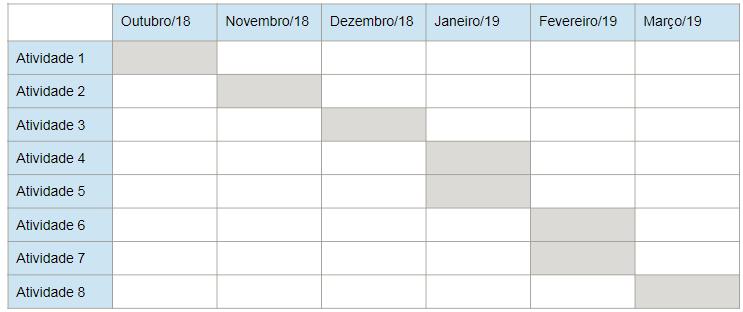
\includegraphics[width=\textwidth]{cronograma_qualificacao1}\\
    Fonte: Autor\hfill
    \label{fig:cronograma}
\end{figure} 



% ---
% Conclusão
% ---
%\chapter*[Conclusão]{Conclusão}
%\addcontentsline{toc}{chapter}{Conclusão}




% ----------------------------------------------------------
% ELEMENTOS PÓS-TEXTUAIS
% ----------------------------------------------------------
\postextual


% ----------------------------------------------------------
% Referências bibliográficas
% ----------------------------------------------------------
\bibliography{abntex2-modelo-references} %% REFERENCIA AO ARQUIVO abntex2-modelo-references.bib

% ----------------------------------------------------------
% Glossário
% ----------------------------------------------------------
%
% Consulte o manual da classe abntex2 para orientações sobre o glossário.
%
%\glossary

% ----------------------------------------------------------
% Apêndices
% ----------------------------------------------------------

% ---
% Inicia os apêndices
% ---
%\begin{apendicesenv}

% Imprime uma página indicando o início dos apêndices
%\partapendices

% ----------------------------------------------------------
%\chapter{}
% ----------------------------------------------------------



%\end{apendicesenv}
% ---


% ----------------------------------------------------------
% Anexos
% ----------------------------------------------------------

% ---
% Inicia os anexos
% ---
%\begin{anexosenv}

% Imprime uma página indicando o início dos anexos
%\partanexos

% ---
%\chapter{.}
% ---


% ---

% ---



% ---


%\end{anexosenv}

%---------------------------------------------------------------------
% INDICE REMISSIVO
%---------------------------------------------------------------------

\printindex

%---------------------------------------------------------------------
% Formulário de Identificação (opcional)
%---------------------------------------------------------------------
%\chapter*[Formulário de Identificação]{Formulário de Identificação}
%\addcontentsline{toc}{chapter}{Exemplo de Formulário de Identificação}
%\label{formulado-identificacao}



\end{document}
